\documentclass[11pt]{article}
\usepackage[margin=1in]{geometry}
\usepackage[T1]{fontenc}
\usepackage[utf8]{inputenc}
\usepackage{lmodern}
\usepackage{amsmath}
\usepackage{booktabs}
\usepackage{graphicx}
\usepackage{caption}
\usepackage{enumitem}
\PassOptionsToPackage{hyphens}{url}
\usepackage[hidelinks]{hyperref}
\usepackage{microtype}

\title{A Seed That Grows by Testing Its Own Changes:\\ Persistent State Improvement Across Five Areas\\ and Three Development Seeds}
\author{Maureese Williams}
\date{October 11, 2026}

\begin{document}
\maketitle

\begin{abstract}
An agent can improve without improving the algorithm that teaches it: it can accumulate evidence, learn where to search, or acquire a primitive that makes a previously inexpressible solution expressible. This paper asks whether one persistent agent, a seed, can combine these forms of growth, decide for itself which changes to its state to keep, and carry that state into settings with different structure. The seed holds a language of atoms from which its hypothesis catalog is built, the experience it has earned by solving tasks, a model of each setting fitted from that experience, and a ledger of every change it tried. After each life of 48 worlds it proposes changes of three kinds, a refit model, invented atoms, and the removal of atoms that never earned their keep, and accepts a change only when the change solves more tasks than the carried state on a held-out set of worlds the seed has never trained on. A change to the shared language must also leave every previously learned setting within a stated tolerance. On held-out sets never used by any acceptance test, the seed on development seed 644101 raised its solve count from 1,232 to 2,072 of 7,200 tasks in family-structured worlds over twelve lives, from 211 to 364 of 2,400 in a random partition of atoms over four lives, from 427 to 2,076 of 4,800 in worlds with behavioural structure over four lives, and from 199 to 360 and 294 to 442 of 2,400 in two further partitions with four and two groups per world. Fresh seeds on 643101 and 645101 rose from 1,372 to 2,006 and from 1,159 to 2,048 in three lives of the first setting. Models were accepted on nearly every life; 111 invented atoms stand in the language, 55 of them reproducing atoms of the two families withheld from the seed; four removals were accepted. The acceptance rule itself had to be revised twice, once when a change accepted in one setting damaged another by 10\%, and once when a change accepted on a small point gain failed to hold. The evidence is development evidence on three opened seeds without a predeclared gate, and the learner code is fixed: what the seed improves is the state that code runs on.
\end{abstract}

\section{Introduction}

An agent can improve its performance without improving the algorithm that teaches it. It can accumulate useful evidence, learn where to search, or acquire a new primitive that makes a previously inaccessible solution expressible. These are different forms of growth. The question here is whether one persistent agent can combine them, decide which changes to retain, and carry the resulting state into settings with different structure.

Each form had been demonstrated separately in this programme, in separate code, with nothing carried between runs except files written by hand. An agent that keeps the atoms of whatever it submits, right or wrong, raises its own solve rate four to ten times across a hundred tasks at every scan budget from 128 to 4,096, and being told whether it was right adds nothing. A grouping of atoms learned without labels from 1,600 worlds solves 6,993 and 8,077 more tasks over 18 budget cells than the same agent on a grouping from 400 worlds, on predeclared seeds, audited. In the string DSL, a system that synthesises primitives from its failures solved 20 of 24 tasks where its fixed grammar solved 5, on two seeds. What the three had in common was a state that grew with experience and a learner that did not, and none was recursive in the programme's sense of a later improver producing a better child improver; every attempt at that returned a null result.

The step taken here is to make the state the object that grows, in one artifact, and to make the artifact decide which changes to keep by one test: a change is kept only if, on worlds the seed has never trained on, drawn fresh for the occasion, it solves more tasks than the state before it, with the cost of the test charged to the seed. This is an empirical acceptance comparison, not a guarantee; the implementation calls the operation \emph{prove} and the paper uses \emph{accept} and \emph{test} for what it does. A seed built this way cannot claim a gain it did not measure, and, after a revision the results forced, it cannot keep a change that helped the setting proposing it by damaging a setting it had learned before.

The paper answers a narrow question. Does one such seed, started with a language that lacks two of the nine atom families and no model of any world, grow across several settings of different structure, and does the growth hold on worlds no acceptance test ever used? It does, on three development seeds. The paper reports how much, what was kept, what was invented, where the design failed and how the acceptance rule was revised, and what the result does not establish.

\section{Setting and vocabulary}

Every setting in this paper shares one hypothesis space and one task form; what differs between settings is the hidden structure that decides which atoms appear together.

\paragraph{Atoms and the catalog.} An \emph{atom} is a predicate on a single character, written in the host language's ordinal expression grammar: for example, that the character's code is 3 modulo 7, or that bit 5 of its code is set. There are 313 atoms in the full set, in 9 \emph{families} named for the arithmetic operation they apply (mod, bit, threshold, popcount, parity, divmod, gcd, xormod, rotmod). The \emph{catalog} is every atom, every pair of atoms from different families under and, or and xor, and every complement of these, reduced to one row per distinct behaviour over the 256-character alphabet. From all 313 atoms it has 166,596 rows. The seed's catalog is built from its own \emph{language}, the atoms it currently holds, and is rebuilt whenever the language changes: 82,758 rows from its starting 260 atoms, 266,272 rows at its largest language of 426 atoms, 208,142 at the 371 atoms it ended with.

\paragraph{Worlds and tasks.} A \emph{world} is a set of 14 atoms; its \emph{mechanisms} are the catalog rows built only from those atoms, about 160 on average, and a world is admitted only if it has at least 130. A \emph{task} is drawn from one mechanism: 8 visible examples, each a string whose longest prefix of characters satisfying the mechanism is the answer, and 16 hidden examples that score the submission. The agent solves a task by scanning the catalog in an order of its own choosing, stopping after a fixed number of rows, the \emph{scan budget}, and submitting the smallest row consistent with the visible examples. A task is solved when the submission also reproduces the hidden examples. The agent is never told whether it did.

\paragraph{Lives, earning, and confident picks.} The agent lives a world as a stream of 100 tasks. Within a world it keeps the atoms of whatever it submits as evidence, and that evidence reorders the catalog for the next task; this is the \emph{earned loop}, and the atoms it accumulates in a world are its \emph{earned} experience of that world. The agent also records, for each submission, how many consistent rows it found inside the budget before submitting. A submission made with exactly one consistent row in the window is correct 90\% of the time, and one made with more than sixteen 26\% of the time; the former are the agent's \emph{confident picks}, and only they feed its models. A \emph{life} is 48 worlds lived in one setting.

\paragraph{Areas.} A \emph{setting}, called an \emph{area} in the implementation, is a generator of worlds: a rule for which atoms appear together. Section~4 describes five. The seed is never told the rule, which family an atom belongs to, or which area a world came from.

\paragraph{The carried state and the acceptance test.} The \emph{carried state} is everything the seed keeps between lives (Section~3). A \emph{candidate} is a proposed state. An \emph{acceptance test} runs the carried state and the candidate on the same held-out worlds, drawn from the area for that test and never lived, and keeps the candidate only if it solves more. The paper's growth numbers come from a further set of held-out worlds that no acceptance test ever used.

\section{The seed}

The seed is one artifact: a state file and four operations that read and rewrite it. Nothing else persists between lives, and nothing in the operations is specific to an area.

\paragraph{State.} The seed carries its language; its experience, one record per world lived, holding the area and the atoms behind its confident picks and behind all its picks, by atom name so that the records survive a change of language; per area, a world and self model and a flag that says whether to build a prior from that area's experience; the atoms it has invented and when they entered; a ledger of every candidate with its test; and the resource it has spent on living, testing and inventing.

\paragraph{Live: earn experience in an area.} The seed draws fresh worlds and lives each as a stream of 100 tasks at the scan budget. Its catalog order is the earned loop's, and two things it carries can reorder it further. When it has a model for the area, a posterior over which groups of atoms the current world uses, updated from the atoms earned so far in that world, lifts the rows those groups build. When it has a prior for the area, the scan starts from an order given by pair co-occurrence in its own earlier worlds there, with half of each task's budget reserved for the order it would use with no prior at all. With neither it scans in catalog order. Each pick is recorded with its count of consistent rows.

\paragraph{Reflect: refit the area's model from everything earned there.} From the area's confident picks the seed fits a world and self model by expectation-maximization, as described in the companion paper: a group label per atom, how often each set of groups occurs, and for each atom a discovery rate, how often the seed finds it when it is present, and an import rate, how often the seed earns it by a wrong pick when it is absent. An atom whose discovery rate falls below 0.10 is filed in no group: the seed meets it only through its own mistakes. The seed fits 6, 7 and 8 groups and 2, 3 and 4 groups per world and keeps the pair with the best likelihood on its last fifth of worlds. The refit model and a prior from the area's experience form one candidate.

\paragraph{Extend: invent atoms for the worlds it could not solve.} For the third of the life's worlds with the most tasks left without any consistent row in the window, and only worlds with at least 15 such tasks, the seed enumerates depth-one expressions from the ordinal grammar, 3,456 candidates distinct up to complement, smallest first, and tests each against the constraints of the unsolved tasks: alone, complemented, or joined by and, or or xor to one atom it earned in that world. A candidate atom is kept when it fits at least two uncovered tasks, because an atom a world is built from recurs across the world's mechanisms and a chance fit does not. Up to 40 new atoms per life form the candidate language.

\paragraph{Prune: propose removing atoms that never earned their keep.} An invented atom is proposed for removal two or more lives after it entered if it has never appeared in a confident pick, or if every area model that has seen it rates it as found only through wrong picks.

\paragraph{Prove: test every candidate before it is kept.} After a life the seed proposes all three kinds of change at once and tests the combination; if the combination fails, it tests each part alone. A test runs the carried state and the candidate on the life's held-out set. Under the rule in force at the end of this work, a candidate is kept only when its gain over the carried state, paired over the held-out worlds, has a 95\% bootstrap interval above zero; a candidate clearly behind on the first half of the set is stopped there. A candidate that changes the language, which every area shares, is also run on a smaller held-out set of each other area the seed has lived in and is dropped if its total there falls more than 2\% below the carried state's (a relative decrease of the total on that set). Every held-out lifetime is charged to the seed's resource. Section~5 gives the history of this rule, which was revised twice.

\begin{figure}[t]
\centering
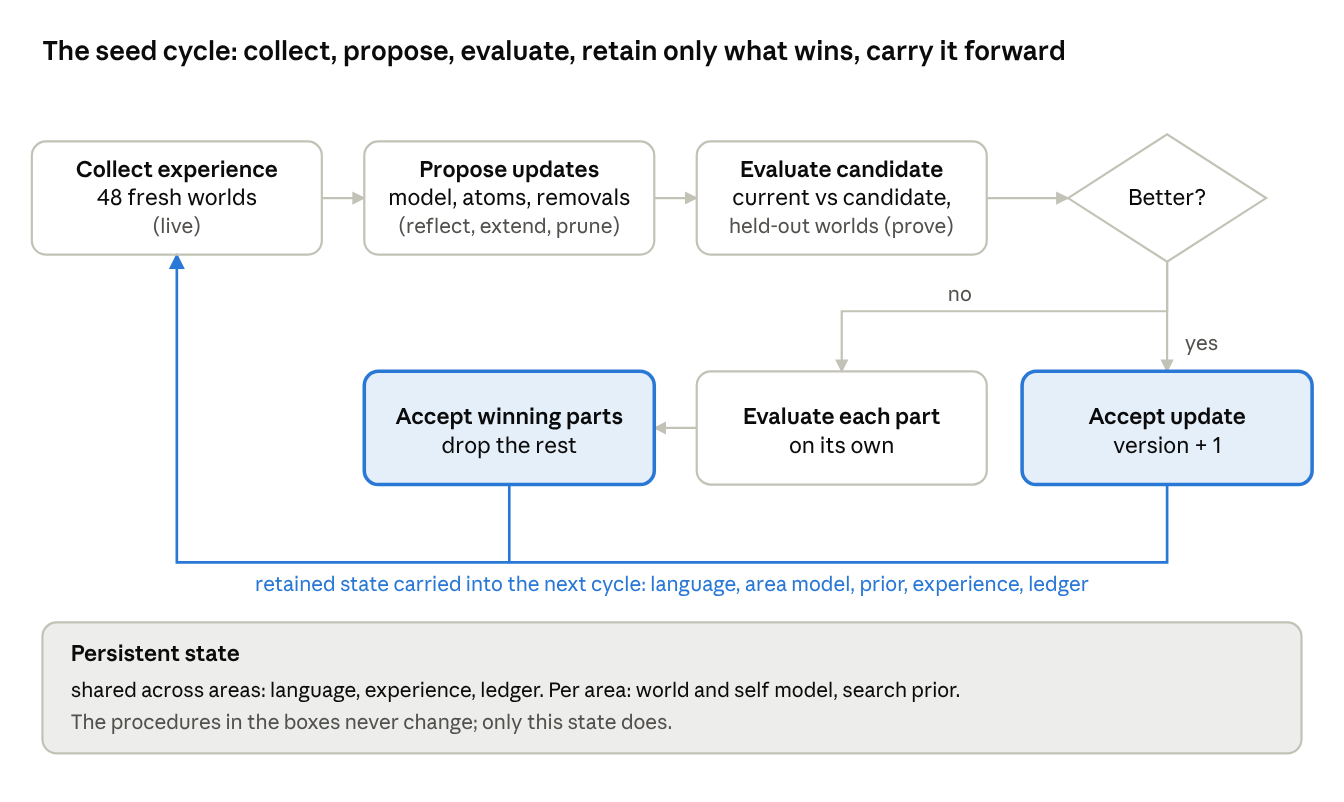
\includegraphics[width=\linewidth]{fig-seed-life.png}
\caption{One life of the seed. It lives 48 fresh worlds, proposes every change it has, tests the combination on a held-out set drawn for that life, keeps it if the combination wins, and otherwise tests each part on its own. A change to the shared language is also run on the other areas the seed has lived in and dropped if it is more than 2\% worse anywhere. Every held-out lifetime is charged to the seed; dropped parts leave only a ledger entry; kept parts are never reset except by a later accepted removal.}
\label{fig:life}
\end{figure}

A life therefore ends with at most three accepted changes and at least one ledger entry (Figure~\ref{fig:life}).

\section{Areas}

\paragraph{Mechanism worlds (\texttt{mech}).} A world draws three of seven families and its 14 atoms from their pooled atoms. The seed's starting language lacks the two remaining families, popcount and xormod, so a world that uses one of them holds mechanisms the seed cannot reach by scanning at any budget. A fifth of the viable family triples are withheld from the seed's lives as \emph{untrained combinations}. Lives draw three quarters of their worlds from trained triples and a quarter from triples with an unfamiliar family; held-out sets hold equal numbers of trained, untrained and unfamiliar worlds.

\paragraph{Drawn partitions (\texttt{drawn7}, \texttt{drawn11}, \texttt{drawn13}).} Every atom of every family is assigned at random to one of a few groups; a world picks some groups and draws its 14 atoms from their union, and each atom slips to a uniformly random atom with some probability. The partition cuts across families, so nothing learned about mechanism worlds applies except the language. The three areas differ in structure: 9 groups with 3 per world and slip 0.15; 12 groups with 4 per world and no slip; 6 groups with 2 per world and slip 0.15. The seed is not told how many groups a world uses.

\paragraph{Metric worlds (\texttt{metric777001}).} Each atom has a behavioural descriptor, the normalised Fourier and Walsh spectra of its truth mask over the alphabet. A sparse weighting over descriptor dimensions is drawn once and shown to nobody. A world is a centre atom together with the atoms nearest it under that weighting, fourteen in all, the centre included as the nearest to itself. A quarter of each life's worlds are centred on an atom of the two families the seed's language lacks. Here the hidden structure is behavioural rather than syntactic.

What the seed carries between areas is its language and its experience. What it fits per area is the model and the prior, because a grouping that explains one area's worlds says nothing about another's. The ledger, the acceptance tests and the resource accounting are shared.

\section{Protocol and chronology}

\paragraph{Schedule.} A life is 48 worlds of 100 tasks at a budget of 1,024 scans per task. The seed's state is saved after every operation, so lives in different areas can be interleaved and a run resumed. Seed \texttt{s1}, on development seed 644101, lived twelve lives in mechanism worlds, four in \texttt{drawn7}, four in \texttt{metric777001}, three in \texttt{drawn11} and two in \texttt{drawn13}, in that order except that mechanism lives 10 and 11 came last. Seeds \texttt{s2} and \texttt{s3}, on 643101 and 645101, lived three mechanism lives each.

\paragraph{Held-out sets.} An acceptance test uses 24 worlds per pool of the area (72 for mechanism worlds, 24 for the single-pool areas), and the cross-area check 12 per pool. From version 11 of \texttt{s1} onward, every life draws its own held-out set; the first eight mechanism lives (versions 0 to 10) reused one fixed set, and the numbers the seed read on it carry the optimism that reuse allows. The growth numbers reported in Section~6 come from one further held-out set per area, drawn with a salt no test ever used, on which the carried state and the starting state (initial language, no model, no prior) are run once each.

\paragraph{The acceptance rule, by version.} The rule changed as the results exposed its weaknesses, and the ledger records which rule accepted each change.

\begin{table}[h]
\centering
\caption{Which acceptance rule was in force for which changes of \texttt{s1}.}
\label{tab:chronology}
\small
\begin{tabular}{p{0.26\linewidth}p{0.68\linewidth}}
\toprule
Versions (lives) & Rule \\
\midrule
0 to 10 (mechanism lives 0 to 7) & Candidate kept if it solves strictly more than the carried state on one fixed held-out set; single-area test; one model for the one area. \\
11 to 22 (mechanism 8 to 9, \texttt{drawn7} 0 to 3, \texttt{metric} 0 to 3) & As above, but the held-out set is drawn fresh for each life and models and priors are kept per area. \\
23 to 25 (\texttt{drawn11} 0 to 2, \texttt{drawn13} 0 to 1, mechanism 10) & Combination tested first, then parts; a language change must also stay within 2\% of the carried state on every other area lived; groups per world chosen by held-out likelihood. \\
26 (mechanism 11) & Candidate kept only if the paired 95\% bootstrap interval of its gain over worlds is above zero; tie-break a hash of row content; prune also on the self model's verdict. \\
after 26 & Half-set early stop and version snapshots for audit; not exercised in the results reported here. \\
\bottomrule
\end{tabular}
\end{table}

\paragraph{What the seed never sees.} It never sees a family label, a true world, an area name except as a key for its own model, which pool a world came from, or whether a submission was correct. It reads its own picks, their consistent-row counts, the tasks with no consistent candidate, and its held-out solve counts. Labels enter only in scoring, to say which pool a world came from and which family an invented atom reproduces.

\paragraph{Resource.} The ledger charges living (worlds $\times$ 100 tasks $\times$ budget scans), every held-out lifetime of every test, and every invention test, so the cost of growing is recorded beside the cost of living.

\section{Results}

\begin{figure}[t]
\centering
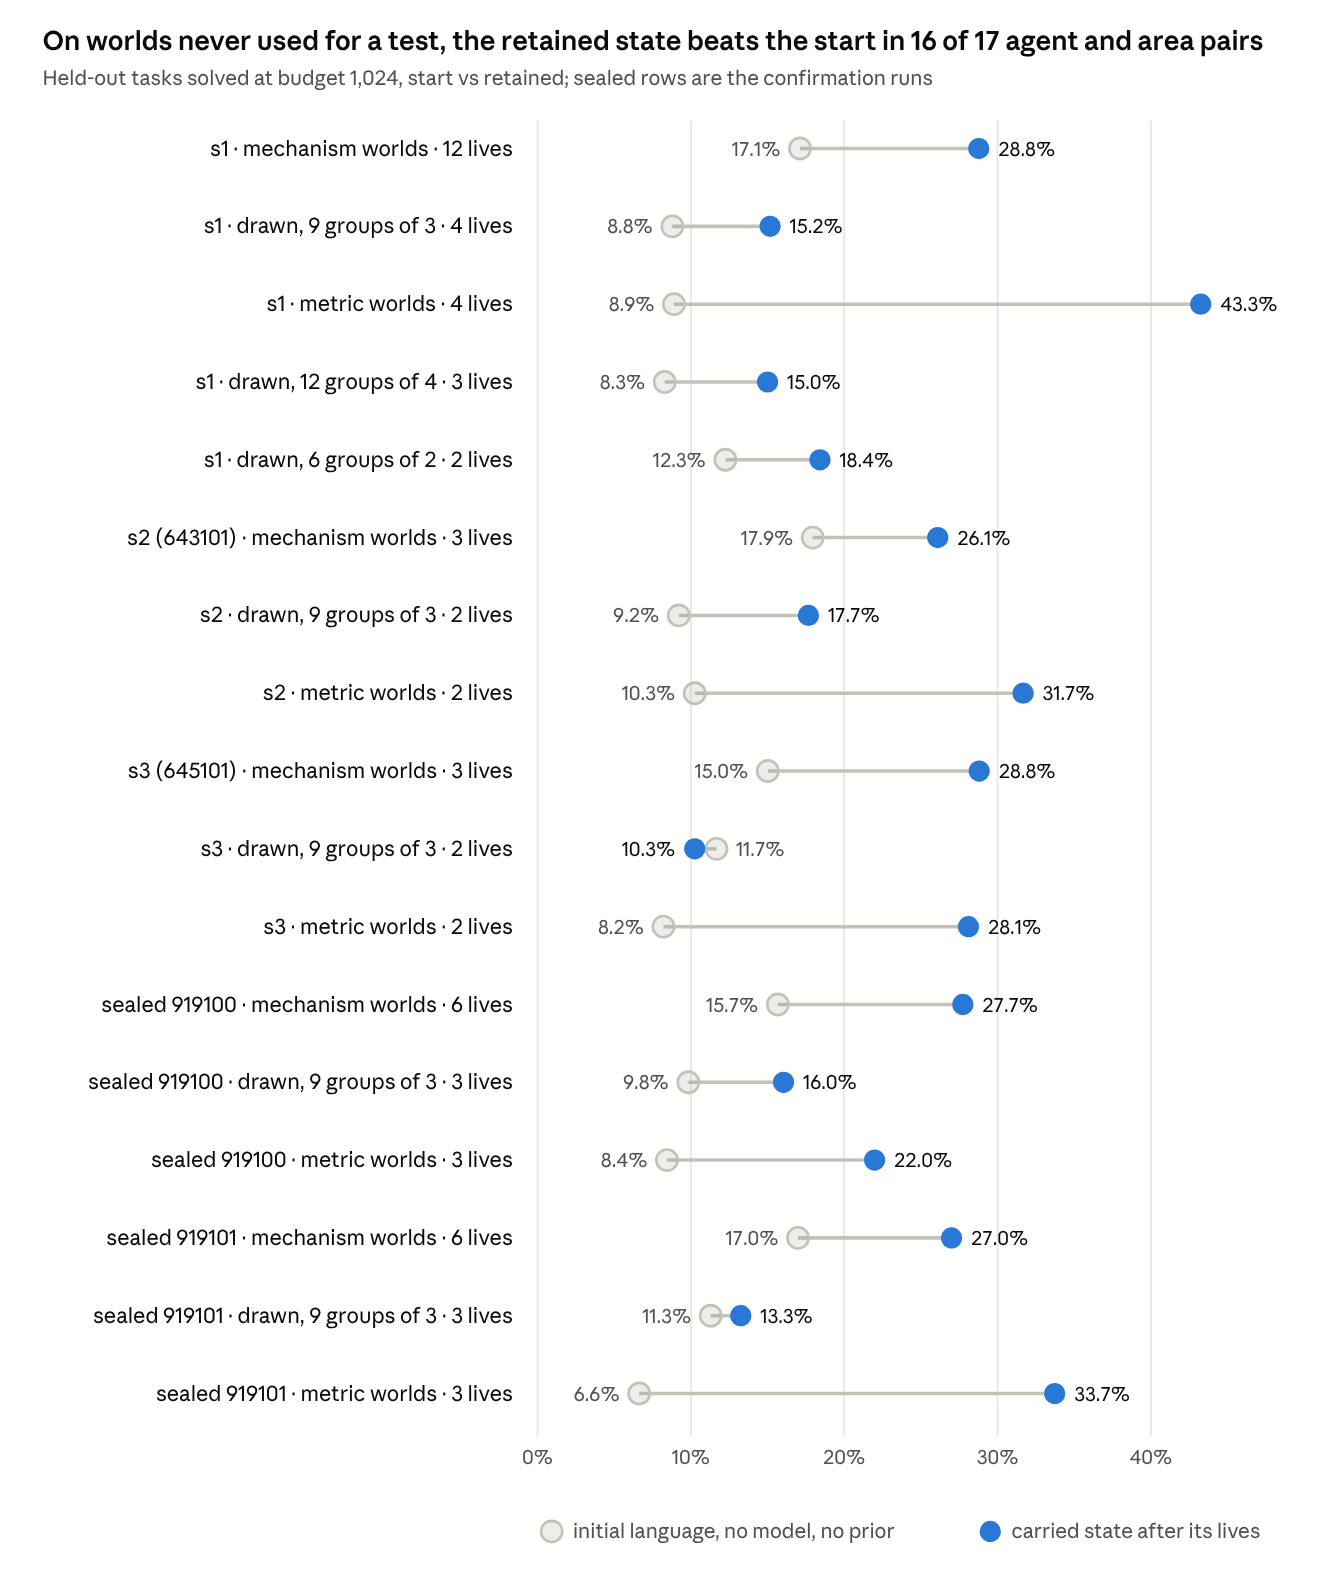
\includegraphics[width=\linewidth]{fig-seed-growth.png}
\caption{Share of held-out tasks solved at budget 1,024 on sets no acceptance test used: the starting state (open) against the carried state (filled), per area and seed. Each point is one draw of 24 worlds per pool; no interval is attached because the check records totals only, a limitation noted in Section~9.}
\label{fig:growth}
\end{figure}

\begin{table}[t]
\centering
\caption{Growth on held-out sets never used by an acceptance test: tasks solved, 24 worlds per pool at budget 1,024. The \texttt{s1} rows are under the content-stable tie-break of version 26; \texttt{s2} and \texttt{s3} under the earlier index tie-break.}
\label{tab:growth}
\begin{tabular}{llrrr}
\toprule
Seed & Area (lives) & Start & Carried & Tasks \\
\midrule
s1 & mechanism worlds (12) & 1,232 & 2,072 & 7,200 \\
s1 & drawn7, 9 groups of 3 (4) & 211 & 364 & 2,400 \\
s1 & metric worlds (4) & 427 & 2,076 & 4,800 \\
s1 & drawn11, 12 groups of 4 (3) & 199 & 360 & 2,400 \\
s1 & drawn13, 6 groups of 2 (2) & 294 & 442 & 2,400 \\
s2 (643101) & mechanism worlds (3) & 1,372 & 2,006 & 7,200 \\
s3 (645101) & mechanism worlds (3) & 1,159 & 2,048 & 7,200 \\
\bottomrule
\end{tabular}
\end{table}

The seed grew in every area it entered and on every seed it was started from (Figure~\ref{fig:growth}, Table~\ref{tab:growth}). In mechanism worlds \texttt{s1} went from 1,232 to 2,072 of 7,200 held-out tasks over twelve lives: trained worlds from 26 to 49 tasks per world, worlds with an unfamiliar family from 5 to 19, and untrained combinations from 20.5 to 18.6, the one pool that did not rise (Section~8). \texttt{s2} and \texttt{s3}, started fresh on other seeds, went from 1,372 to 2,006 and from 1,159 to 2,048 in three lives. In the first drawn partition \texttt{s1} went from 211 to 364 of 2,400, and in metric worlds from 427 to 2,076 of 4,800, where a model fitted from the first 48 worlds was alone worth 975 tasks on that life's held-out set. In the two later partitions it went from 199 to 360 and from 294 to 442 of 2,400 in three and two lives, keeping one model in each; for the first it chose four groups per world, that area's true structure, and for the second also four, where the truth is two.

\paragraph{What was accepted.} Over 26 versions \texttt{s1} kept 16 models, 6 language extensions and 4 removals, and dropped 18 extensions, 6 models and 1 removal. A model was kept on every mechanism life from 0 to 6, with gains on the seed's own held-out sets of 417, 118, 13, 133, 98, 2 and 11 tasks; on lives 8 and 9 no model passed. In \texttt{drawn7} a model was kept on the first three lives and a removal on the first and fourth; in metric worlds a model on three lives of four, an extension on the second and a removal on the fourth; in the two later partitions one model each. On \texttt{s2} and \texttt{s3} a model was kept on all three lives (gains 475, 50, 59 and 412, 74, 118) and every extension was dropped. The gains before version 26 are point differences on 24 to 72 worlds and carry no interval; the model line is the consistent one, and invention pays off only sometimes, with smaller gains.

\paragraph{What was invented.} At version 17 the language held 151 invented atoms: 25 reproduced true popcount atoms and 28 true xormod atoms, the two families withheld from the seed, and 98 were atoms of no family, behaviourally new. By version 24 the count was 166 (27, 29 and 110). At version 26, after the seed removed 55 atoms that every area model rated as found only through its own wrong picks, 111 remain: 26 popcount, 29 xormod and 56 behaviourally new. Invented atoms entered only through an accepted test, and the seed's own removals took out 23, 26, 25 and 55 of them in four accepted steps. On mechanism worlds with an unfamiliar family, where the starting language cannot express a third of the mechanisms, invention is the only route to the rise from 5 to 19 tasks per world.

\paragraph{What it cost.} By version 26 \texttt{s1} had spent 122.9 million scans living, 302.3 million scans testing, and 831,738 invention tests. Testing cost two and a half times living, because each life tested up to four candidates on 72 worlds against a freshly scored carried state, and the cross-area checks added to that. The ratio is the first thing to cut; it does not change what was kept.

\paragraph{What the seed read against what held.} The per-life held-out totals the seed decided by were, on the fixed set of the first eight mechanism lives, 1,291, 1,708, 1,722, 1,840, 1,853, 1,898, 2,031, 2,129, 2,131, 2,142 and 2,195, and on fresh sets thereafter 2,234, 2,089, 2,401, 2,425 and 2,008. The untouched set gave 2,072 for the carried state. The numbers the seed decided by and the numbers that held are within a few percent of each other, with one exception that changed the rule: on life 10 a model was kept for a gain of 24 on that life's set and read 82 lower on the untouched set.

\section{Interference across areas}

A change can improve the area that proposes it while damaging an area the seed has already learned. The first three-area check exposed exactly this failure.

After four lives in metric worlds, \texttt{s1}'s score on the first drawn partition's untouched held-out set fell from 376 to 338, a 10\% loss in an area it had not entered since. The cause was the shared language. The metric lives had accepted one extension of 40 atoms and one removal of 25, each tested on the metric area alone, and a language that grew and shrank to suit metric worlds changed the catalog the drawn partition's model had been fitted over. Each change was an accepted success where it was tested and a regression where it was not.

The revision is to the acceptance rule, not to the areas. From version 23, a candidate that changes the language is also run on a held-out set of every other area the seed has lived in, 12 worlds per pool, and is dropped if its total there falls more than 2\% below the carried state's. The carried scores of those areas are recomputed after any accepted shared change, so no later test compares against a stale number. The tolerance permits a small measured regression; it is a bound, not preservation. The cost is more held-out lifetimes per language candidate, which is why the combination of all proposals is tested first and the parts only if it fails.

The revised rule fired twice as soon as it existed. In \texttt{drawn11} a combination of invented atoms and a model gained 165 to 344 on that area's held-out set and was dropped because it cost mechanism worlds 8\% and \texttt{drawn7} 12\%; the model alone was then kept, at 417. In \texttt{drawn13} a combination worth 150 was dropped for costing \texttt{drawn11} 23\%. Each would have been an accepted success under the earlier rule.

\section{The grown language and the pools the seed cannot see}

A second weakness showed in the five-area check at version 24, on the mechanism area's untouched set: untrained family combinations had fallen from 24 to 18 tasks per world while trained worlds rose from 26 to 50. The acceptance tests had not seen it, because a test compares totals and the untrained pool is a third of the set.

An ablation of the carried state on that set attributes the loss (Table~\ref{tab:ablation}). The carried model and prior on the starting language score 1,973 with untrained combinations at 26 per world, above the start; the grown language alone, with no model and no prior, scores 735 against 1,299 for the starting language; the carried state scores 2,072 with untrained at 18. The 166 invented atoms, 110 of them behaviourally new, had enlarged the catalog from 82,758 rows to 266,272, and the half of each task's budget that the prior rule reserves for the no-prior order was scanning a catalog two thirds of which the seed had added. Trained worlds did not suffer, because the model's half of the budget found their rows anyway; untrained combinations, which the model lifts less, did.

\begin{table}[t]
\centering
\caption{Ablation of \texttt{s1}'s carried state (version 24) on the mechanism area's untouched held-out set: tasks per world by pool, and total of 7,200.}
\label{tab:ablation}
\begin{tabular}{lrrrr}
\toprule
State & Trained & Unfamiliar & Untrained & Total \\
\midrule
carried & 49.5 & 18.7 & 18.2 & 2,072 \\
carried, no prior & 43.0 & 14.7 & 9.5 & 1,614 \\
carried, no model & 37.3 & 15.0 & 15.9 & 1,639 \\
grown language only, no model, no prior & 11.1 & 9.0 & 10.5 & 735 \\
starting language, carried model and prior & 50.0 & 6.1 & 26.2 & 1,973 \\
starting state & 26.2 & 3.7 & 24.2 & 1,299 \\
\bottomrule
\end{tabular}
\end{table}

The seed already held the verdict it needed. Its self model files an atom in no group when the seed would almost never find it in a world, which means the atom is met only through wrong picks. Across the five area models, 107 invented atoms were rated real by at least one model, 55 of the 56 that reproduce a withheld family among them, and 59 were rated import-only by every model that had seen them, one of them real. From version 26 the prune operation proposes those too, and the acceptance test decides.

Two further revisions went in at the same version, both to the test. On life 10 a model had been kept for a gain of 24 on that life's set and read 82 lower on the untouched set, so a candidate is now kept only when its paired gain over the held-out worlds has a 95\% bootstrap interval above zero. And the tie-break, the order the scan uses among rows it scores equally, had been a random permutation of row indices, so adding or removing any atom reshuffled every other row and every language test carried that noise; it is now a hash of each row's content, so a language change changes nothing but the rows it adds or removes.

On life 11 the removal of the 55 atoms was accepted, +0.3 to +3.0 tasks per world on the mechanism set and better in all four other areas, and the model and extension proposed beside it were dropped on intervals that crossed zero. The language went from 426 to 371 atoms. On the untouched set untrained combinations now read 18.6 against a start of 20.5, inside the 10\% that the draft confirmation protocol allows, with every other pool and area above its start.

\section{What this does and does not show}

It shows one artifact improving its own state in five areas of different structure and on three seeds, keeping only changes it tested on worlds it never trained on, with the tests charged. The three forms of growth the programme had reproduced separately appear together in its ledger: the earned loop inside every life, the model and prior that were accepted nearly every life and account for most of the gain, and the invented atoms that let it reach families its starting language could not express. Growth in one area did not require starting over in another; the language carried, and in the metric area a model fitted from 48 worlds was worth 975 tasks at once.

It is development evidence. The seeds were opened, no gate was predeclared, no forecast was committed, and nothing was audited by independent replay. The held-out sets behind Table~\ref{tab:growth} were never used by an acceptance test, which is the one protection against the seed having tuned itself to its own scoreboard; but each is a single draw whose per-world results were not saved, so no interval accompanies those totals. Version snapshots and an auditor that replays accepted tests exist from version 26 on and have not yet been run.

It is recursive in one sense and not in another. The seed's model and language direct its earning, its earning produces the experience the next model and language are fitted from, and the ledger shows the state improving the state across twelve lives. But the operations that turn experience into a model, candidates into atoms, and tests into acceptances are fixed code. A later seed does not produce a better reflect or a better extend, and the programme's definition of recursive growth, a later improver producing a better child improver, is not met.

The growth also saturates and is uneven. On \texttt{s1}'s later mechanism lives few candidates passed, and model gains fell from hundreds to single digits by the sixth life. Untrained combinations in mechanism worlds ended 9\% below their start. Half of the remaining invented atoms are behaviourally new and some are surely junk that costs scan budget until a removal takes them out. Testing cost two and a half times living. And every area shares one task form and one catalog; the seed has not met a second domain.

\section{Lessons}

\begin{enumerate}[leftmargin=*]
\item The acceptance test is the seed. Every design choice that mattered concerned what counts as an accepted change: a paired interval above zero on a fresh held-out set, within tolerance everywhere the state is shared, cost charged. Given that rule, a weak candidate costs a test and nothing else, so the seed can propose freely.
\item Test the combination first, then the parts. This halved the tests in the common case and lost nothing, because a combination that wins is kept whole.
\item Invention needs recurrence. An atom that fits one unsolved task is usually a coincidence; one that fits two is usually a missing atom. The first version accepted single fits, and every extension it proposed lost.
\item Let the seed remove what it added. Removing atoms that never earned their keep was accepted three times in three, and removing the atoms the self model called import-only recovered a loss no test had seen.
\item A model from 48 worlds can be worth keeping. The programme's earlier rule that a prior fitted on 25 worlds is worse than none was read on handed atom sets at tight budgets; here, with the test deciding, the first model was accepted on every seed and every area.
\item Shared state needs shared tests. The 10\% loss in an untouched area was invisible to any single-area test.
\item Score growth on worlds the seed never saw, and attach an interval. A gain of 24 on 72 worlds is noise.
\item Make the measurement stable under the change being measured. A tie-break drawn over row indices turned every language change into a reshuffle of the whole catalog.
\item Build for the host. One stall and one crash in the record were the machine's shared memory, not the seed; retries with fewer workers and periodic stack dumps cost nothing.
\end{enumerate}

\section{Next}

\begin{itemize}[leftmargin=*]
\item Confirmation. A predeclared gate on sealed seeds: after a fixed schedule of lives in three areas, the carried state beats the starting state on fresh held-out sets by a stated margin in every area, no pool falls below 90\% of its start, testing costs at most 2.5 times living, and every accepted change replays. The draft protocol exists; it is not frozen.
\item Intervals on the growth numbers. The untouched checks should save per-world results so that Table~\ref{tab:growth} carries intervals.
\item Testing cost. The half-set early stop is in; smaller cross-area sets are the next cut, and the aim is a cost below living without changing what is accepted.
\item Pools the seed cannot see. The untrained-combination loss was mostly the grown language, and the seed's verdict on its own atoms removed most of it; a label-free guard on the no-prior half of the budget remains the place to look if it returns.
\item More areas and a second domain. A second task form and a second alphabet in the same catalog come first, then the string DSL banks, which require the seed's solver to be one of several rather than the one it has.
\item The next level. The seed improves its state, not its operations. The first operation it could plausibly improve is the acceptance test itself, learning from its ledger how large a held-out set each kind of candidate needs. The ledger is the first data such a learner could be fitted on.
\end{itemize}

\section{Reproducibility}

The repository is the RSI project at \path{projects/rsi}. The seed is \path{rsi/seed.py} (state, areas, the four operations, the acceptance test) with \path{rsi/seed_areas.py} for metric worlds, \path{rsi/invention.py} for the grammar and the recurrence test, and \path{rsi/self_world_model.py} for the model. \path{seed_run.py --name s1 --seed 644101 --area mech --lives 4} runs lives and resumes from the saved state; \path{seed_check.py --name s1 --areas mech,drawn7,metric777001} scores a seed on held-out sets no test used and labels its inventions; \path{seed_ablate.py} produced Table~\ref{tab:ablation}; \path{audit_seed.py} replays accepted tests from version snapshots. States are in \path{seeds/<name>/state.json}, committed after every run; the ledger inside each is the full record of every candidate, its test and its cost. Logs are \path{runs_seed_*.log} and the checks \path{analysis/seed-check-<name>.json}.

Settings: 48 worlds of 100 tasks per life; budget 1,024 scans per task; 24 worlds per pool for an area's held-out set and 12 for the cross-area check; tolerance 2\% relative; group counts 6 to 8 and 2 to 4 groups per world by held-out likelihood; extension cap 40 atoms per life with recurrence 2; removal after 2 lives or on the self model's import-only verdict; tie-break a content hash per row with seed 77; a change kept only when the paired 95\% bootstrap interval (4,000 draws) of its gain is above zero. Area specifications are stored in the state so that a test can rebuild any area the seed has lived in. \path{RSI_WORKERS} caps the worker pool; six or fewer is safe on this machine beside other jobs.

Seeds: \texttt{s1} on 644101 (versions 1 to 26 reported here), \texttt{s2} on 643101 and \texttt{s3} on 645101. The companion paper on the world and self model is \path{SELF-SIMULATION-WORLD-MODEL-2026-10-10.md}, the distillation of earlier growth results is \path{GROWTH-DISTILLATION-2026-10-10.md}, and a living copy of this paper is at \url{https://claude.ai/code/artifact/ebd48ba7-84b1-4bb2-b2e5-eb18375651bc}.

\end{document}
